\newcommand{\figureInterruptTimerOverflow}[1]{
  \def\lang{\detokenize{#1}}
  \def\langRu{\detokenize{ru}}
  \def\langEn{\detokenize{en}}
  \def\figureCaption{XXX: No translation.}
  \ifx \lang\langRu
  \def\figureCaption{
    Срабатывание 8-битного таймера по переполнению.
  }
  \fi
  \ifx \lang\langEn
  \def\figureCaption{
    8-bit timer overflow trigger.
  }
  \fi
  \begin{figure}[H]
    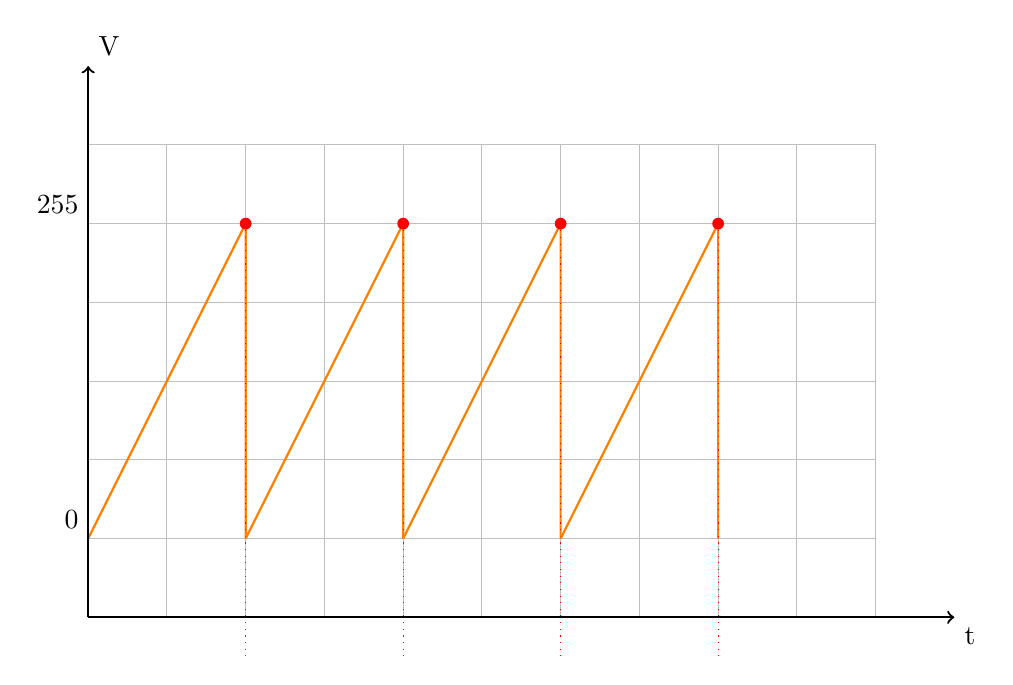
\begin{tikzpicture}
      \draw[lightgray] (0, 0) grid (10, 6);
      \draw (0, 1) node[anchor=south east] {0};
      \draw (0, 5) node[anchor=south east] {255};
      \foreach \x in {0, 2, ..., 6} {
        \draw[thick, orange] (\x,  1)
        -- (\x + 2, 5)
        -- (\x + 2, 1);
        \draw (\x + 2, 5) node[circle,fill,inner sep=1.5pt, red]{};
        \draw[dotted, red] (\x + 2, 5) -- (\x + 2, -0.5);
      };
      \draw[thick, ->] (0, 0) -- (11, 0) node[anchor=north west] {t};
      \draw[thick, ->] (0, 0) -- (0,  7) node[anchor=south west] {V};
    \end{tikzpicture}
    \caption{\figureCaption}
    \label{fig:timer-overflow-interrupt}
  \end{figure}
}
